%\pagestyle{fancy}
\chapter{Methods}
\label{ch:Methods}
Lorem ipsum dolor sit amet, consetetur sadipscing elitr, sed diam nonumy eirmod tempor invidunt ut labore et dolore magna aliquyam erat, sed diam voluptua.
At vero eos et accusam et justo duo dolores et ea rebum. Stet clita kasd gubergren, no sea takimata sanctus est Lorem ipsum dolor sit amet.
Lorem ipsum dolor sit amet, consetetur sadipscing elitr, sed diam nonumy eirmod tempor invidunt ut labore et dolore magna aliquyam erat, sed diam voluptua.
At vero eos et accusam et justo duo dolores et ea rebum. Stet clita kasd gubergren, no sea takimata sanctus est Lorem ipsum dolor sit amet.
Lorem ipsum dolor sit amet, consetetur sadipscing elitr, sed diam nonumy eirmod tempor invidunt ut labore et dolore magna aliquyam erat, sed diam voluptua.
At vero eos et accusam et justo duo dolores et ea rebum. Stet clita kasd gubergren, no sea takimata sanctus est Lorem ipsum dolor sit amet.

\section{IMU only}
\subsection{Calibration}
Because the measurements of the IMU are measured in the coordinate frame of the IMU $\mathcal{I}$, which is not aligned with the car frame $\mathcal{C}$, they have to be transformed.
This can be achieved using a rotation matrix \mtf{i}{c} which transforms the measurements of the linear acceleration $\vincs{a}{I}_n \in \mathbb{R}^{1\times3}$ and angular velocity ${\vincs{v}{I}_n \in \mathbb{R}^{1\times3}}$ into the car frame. $n \in \mathbb{N}$ is the time step.

\begin{figure}[htb]
	\centering
	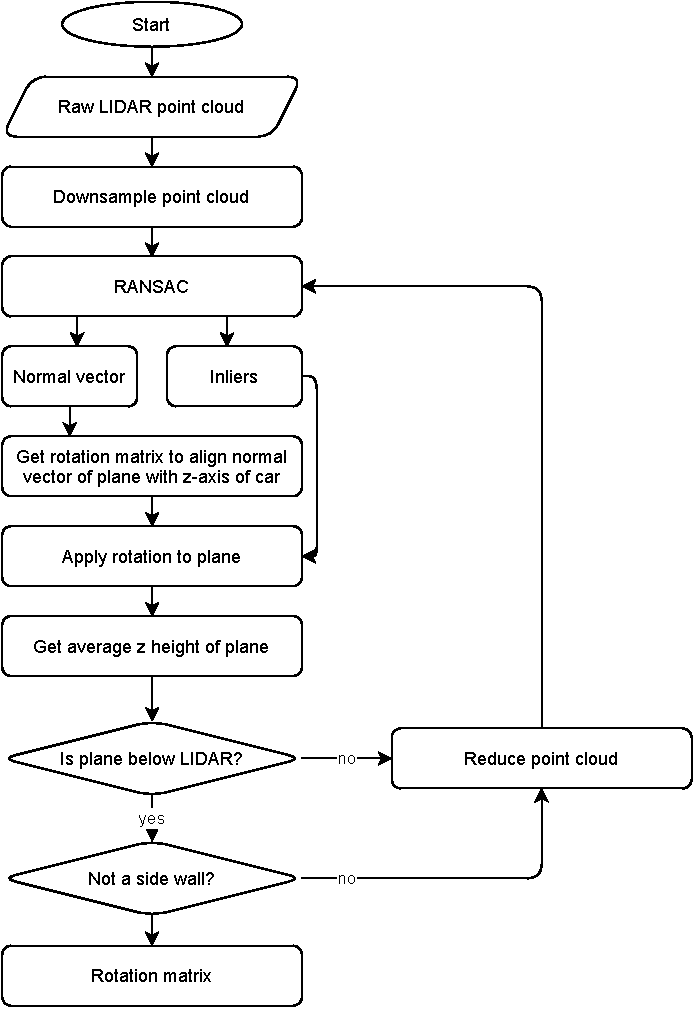
\includegraphics[width=0.7\linewidth]{lidarCalibration.pdf}
	\caption{Algo for lidar alignment}
	\label{fig:lidarCalibration}
\end{figure}

During standstill, the only measurable acceleration besides noise and bias is the acceleration due to gravity.
Assuming the car stands on flat ground, the gravity acceleration in the car frame is measured in upwards z-direction.
In a first step, the measured linear acceleration (gravity) in the IMU frame will be aligned with the z-axis of the car.
According to Euler's rotation theorem, which says that any arbitrary rotation of a rigid body while holding one point (origin) fixed can be achieved by a rotation around a single fixed axis passing through the origin, there exists one rotation axis $\mathbf{j}$ and rotation angle $\alpha$ to achieve this.\\
In the first step, a quaternion \qtf{i}{b} which transforms the measurements from the device frame $\mathcal{I}$ to an intermediate coordinate system $\mathcal{B}$, which has the z-axis up, will be found.
Resulting in $\vincs{z}{b} = \vincs{z}{c} = \mathbf{e}_\mathrm{z} = \left(\begin{array}{lll} 0 & 0 & 1 \end{array}\right)^{\top}$.
This usually is not the case for the other axes $\vincs{x}{b}\neq\vincs{x}{c}$ and $\vincs{z}{b}\neq\vincs{z}{c}$.
Using linear algebra \todo{better explaination} the rotation axis $\vb{j}$, which is perpendicular to \dots, can be found with
\begin{equation}
    \vb{j} = \frac{\vincs{\vu{a}}{i} \vdot \vincs{a}{c}}{\norm{\vincs{\vu{a}}{i} \cp \vincs{a}{c}}}
    = \frac{\vincs{\vu{a}}{i} \vdot \vb{e}_\mathrm{z} }{\norm{\vincs{\vu{a}}{i} \cp \vb{e}_\mathrm{z}}}
    = \frac{\vincs{\vu{a}_\mathrm{z}}{i}}{\norm{\vincs{\vu{a}_\mathrm{y}}{i}\vb{e}_\mathrm{x} - \vincs{\vu{a}_\mathrm{x}}{i}\vb{e}_\mathrm{y}}}
\end{equation}
with $\mathbf{a} \in \mathbb{R}^{1\times3}$ being the measured linear acceleration (average) in the IMU or car frame respectively and $\vu{a}$ being the unit vector of it.\\
The rotation angle can be calculated using
\begin{equation}
    \tan(\alpha) = \frac{\norm{\vincs{\vu{a}}{i} \cp \vincs{a}{c}}}{\vincs{\vu{a}}{i} \vdot \vincs{a}{c}} \implies
    \alpha = \arctan(\frac{\norm{\vincs{\vu{a}}{i} \cp \vincs{a}{c}}}{\vincs{\vu{a}}{i} \vdot \vincs{a}{c}})
\end{equation}
resulting in the quaternion
\begin{equation}
    \qtf{i}{b} =
    \begin{bmatrix}
        \vb{j}\vdot\sin(\frac{\alpha}{2}) \\
        \cos(\frac{\alpha}{2})
    \end{bmatrix}
\end{equation}
\itodo{Decide for a notation (w,x,y,z is more common I think)}

Now that the z-axes of both frames are aligned, the x- and y-axis can be aligned by a rotation around the z-axis.
To find this rotation angle $\beta$, the car has to be accelerated forward.
Then different rotation angles will be tested (brute-forced) until only the x-axis will measure an acceleration.
The resulting quaternion \qtf{b}{c} can then be concatenated with the previous quaternion to get the final quaternion
\begin{equation}
    \qtf{i}{c} = \qtf{b}{c} \otimes  \qtf{i}{b}
\end{equation}
A quaternion of the form
$\mathbf{q} = \left[\begin{array}{llll} w & x & y & z \end{array}\right]^{\top}$
can be converted to a rotation matrix with
\begin{equation}
    % { }_{\mathcal{C}}^{\mathcal{I}} \mathbf{M} =
    \mathbf{M} =
    \left[
        \begin{array}{ccc}
            1-2 y^{2}-2 z^{2} & 2(x y-z w) & 2(x z+y w) \\
            2(x y+z w) & 1-2 x^{2}-2 z^{2} & 2(y z-x w) \\
            2(x z-y w) & 2(y z+x w) & 1-2 x^{2}-2 y^{2}
        \end{array}
        \right]
    \end{equation}
And finally the measurements $\mathbf{A}$ can be transformed using
\begin{equation}
    \vincs{A}{c} = \mtf{i}{c} \vdot \vincs{A}{i}
\end{equation}

$\mathbf{j} \in \mathbb{R}^{1\times3}$, $\alpha \in \mathbb{R}$, $\mathbf{A} \in \mathbb{R}^{n\times3}$ with $n$ measurements, $\mathbf{M} \in \mathbb{R}^{3\times3}$

% \begin{equation}
%     { }_{\mathcal{C}}^{\mathcal{I}} \mathbf{p}
% \end{equation}
% which means "p-$\mathcal{I} \text{ in } \mathcal{C}-\text{coordinates}$"
% A rotation matrix ${ }_{\mathcal{C}}^{\mathcal{I}}\mathbf{M}$ that transforms the measurements ${}_{\mathcal{I}}\mathbf{p}$ from the IMU frame to the car frame
% \begin{equation}
%     { }_{\mathcal{C}}\mathbf{p} = { }_{\mathcal{C}}^{\mathcal{I}}\mathbf{M} {}_{\mathcal{I}}\mathbf{p} \quad \forall_{\mathcal{I}} \mathbf{p} \in \mathbb{R}^{3}
% \end{equation}

Einspurenmodell:
\dots give the wheel speeds. To get the car velocity from the individual wheel speed measurements one can use a \dots model.

\begin{align}
    v_\mathrm{car}(t) &= \frac{v_\mathrm{rear,left} + v_\mathrm{rear,right}}{2}\cdot\cos(\gamma) \\
    \alpha(t) &= \frac{v_\mathrm{rl} - v_\mathrm{rr}}{d} \\
    \gamma(t) &= \frac{\alpha}{f_\mathrm{odom}}
\end{align}
\itodo{better explaination}
with $v_\mathrm{rl} \text{ and } v_\mathrm{rr}$ being the wheel speeds of the rear right and rear left wheel respectively. $\gamma$ is the yaw angle of the car, and $\alpha$ ?, $d$ the wheelbase.\\
The car's acceleration
\begin{equation}
    a_\mathrm{car}(t) = \dv{t}v_\mathrm{car}
\end{equation}
but because discrete numerical differentiation e.g. forward difference with step size $h$
\begin{equation}
    a_\mathrm{car}(h) = \frac{v_\mathrm{car}(x + h) - v_\mathrm{car}(x)}{h}
\end{equation}

\begin{figure}[htpb]
    \centering
    \begin{tikzpicture}[scale=1]
        % Car height
        \def\ch{2}
        % Car length
        \def\cl{5}
        % Car body height
        \def\bh{\ch*0.65}
        % Roof length
        \def\rl{\cl*0.6}
        % Roof height
        \def\rh{\ch*0.35}
        % Car tilt angle
        \def\ct{6}
        % Anchor point is southwest
        \coordinate (b) at (0,0);
        % Offset to roof and wheels
        \coordinate (r) at ($(b) +(\cl*0.17,\ch*0.65)$);
        \coordinate (w) at ($(b) + (\cl*0.25,0)$);

        % Body
        \draw[black, fill=black!17, rounded corners=1.2ex, very thick]
        (b) -- ++(0,\bh) -- ++(\cl*1/5,0) --  ++(\cl*3/5,0) -- ++(\cl*1/5,-\bh*0.25)
        -- ++(0, -\bh*0.75) -- (b) -- cycle;
        % Roof
        \draw[very thick, rounded corners=0.5ex, fill=black!20!blue!20!white,thick]
        (r) -- ++(0.2*\rl,\rh) -- ++(0.5*\rl,0) -- ++(0.3*\rl,-\rh) -- (r);
        % \draw[thick] ($(r) + (\cl*0.5,\bh)$) -- ++(0,\rh);
        \draw[thick] (r)++(\rl*0.6,0) -- ++(0,\rh);

        % Wheels
        \draw[draw=black,fill=gray!50,thick] (w) circle (.5);
        \draw[draw=black,fill=gray!50,thick] (w) ++(\cl*0.55,0) circle (.5);
        % Inner wheels
        \draw[draw=black,fill=gray!80,semithick] (w) circle (.35);
        \draw[draw=black,fill=gray!80,semithick] (w) ++(\cl*0.55,0) circle (.35);

        % Car middle point
        \coordinate (m) at (\cl*0.5, \bh*0.5);
        \filldraw (m) circle (2pt) node[below] {car ($\mathcal{C}$)};
        % Coordinate frames
        \draw[thick,->, red] (m) -- ++(1,0,0) node[anchor=north east]{$x$};
        \draw[thick,->, black!35!green] (m) -- ++(0,0,-1) node[anchor=west]{$y$};
        \draw[thick,->, blue] (m) -- ++(0,1,0) node[anchor=south]{$z$};

        % IMU middle point (random)
        \begin{scope}[rotate=15]
            \coordinate (mi) at (\cl*0.2, \bh*0.5);
            \filldraw (mi) circle (2pt) node[below left] {IMU ($\mathcal{I}$)};
            % Coordinate frames
            \draw[thick,->, red] (mi) -- ++(1,0,0) node[anchor=north east]{$x$};
            \draw[thick,->, black!35!green] (mi) -- ++(0,0,-1) node[anchor=west]{$y$};
            \draw[thick,->, blue] (mi) -- ++(0,1,0) node[anchor=south]{$z$};
        \end{scope}
	\end{tikzpicture}
	\caption{Coordinate frames (graphic might not be necessary)}
\end{figure}

\begin{figure}[htpb]
    \centering
	\begin{tikzpicture}[scale=1]
		% RAMP
        % Define/Calc ramp parameters
        % Ramp length
        \def\rl{10};
        % Ramp angle [deg]
        \def\ra{15};
        % Ramp height
        \def\rh{{tan(\ra)*\rl}};

		% Define the points
		\coordinate (A) at (0,0);
		\coordinate (B) at ($(A) + (\rl,0)$);
		\coordinate (C) at ($(B) + (0,\rh)$);
        % Draw and fill ramp
		\filldraw[draw=black, fill=lightgray!25] (A) -- (B) -- (C) -- cycle;

        % CAR
        % Tilt whole car
        \begin{scope}[scale=0.7, xshift=\rl*0.5 cm, yshift=1.9 cm, rotate=\ra]
            % Car height
            \def\ch{2}
            % Car length
            \def\cl{5}
            % Car body height
            \def\bh{\ch*0.65}
            % Roof length
            \def\rl{\cl*0.6}
            % Roof height
            \def\rh{\ch*0.35}
            % Car tilt angle
            \def\ct{6}

            % Anchor point is southwest
            \coordinate (b) at (0,0);
            % Offset to roof and wheels
            \coordinate (r) at ($(b) +(\cl*0.17,\ch*0.65)$);
            \coordinate (w) at ($(b) + (\cl*0.25,0)$);
            % Body
            \draw[black, fill=black!17, rounded corners=1.2ex, very thick]
            (b) -- ++(0,\bh) -- ++(\cl*1/5,0) --  ++(\cl*3/5,0) -- ++(\cl*1/5,-\bh*0.25)
            -- ++(0, -\bh*0.75) -- (b) -- cycle;
            % Roof
            \draw[very thick, rounded corners=0.5ex, fill=black!20!blue!20!white,thick]
            (r) -- ++(0.2*\rl,\rh) -- ++(0.5*\rl,0) -- ++(0.3*\rl,-\rh) -- (r);
            \draw[thick] (r)++(\rl*0.6,0) -- ++(0,\rh);

            % % Car middle point
            \coordinate (m) at (\cl*0.5, \bh*0.5);
            \node at (m) {\textbullet};
            % Wheels
            \draw[draw=black,fill=gray!50,thick] (w) circle (.5);
            \draw[draw=black,fill=gray!50,thick] (w) ++(\cl*0.55,0) circle (.5);
            % Inner wheels
            \draw[draw=black,fill=gray!80,semithick] (w) circle (.35);
            \draw[draw=black,fill=gray!80,semithick] (w) ++(\cl*0.55,0) circle (.35);

            % Draw car acceleration
            \draw[blue, thick, ->] (m) -- ++(3,0) node[anchor=north]{$a_\mathrm{x}$};
            % Gravity vectors
            % Length of g vector
            \def\gl{3}
            % Length of g vector components
            \def\gxl{{\gl*sin(\ra)}}
            \def\gzl{{\gl*cos(\ra)}}
            % Draw vectors
            \draw[red, ->, very thick, rotate=-\ra] (m) -- ++(0,\gl) node[anchor=south west, black](g_end){$\mathbf{g}$};
            \draw[red, thin, ->] (m) -- ++(\gxl,0) node[anchor=north]{$g_\mathrm{x}$};
            \draw[red, thin, ->] (m) -- ++(0,-\gzl) node[anchor=east]{$g_\mathrm{z}$};
            \draw[red, dotted] ($(m)+(\gxl,0)$) -- ++(0,\gzl) -- ++(-\gxl,0);
        \end{scope}
	\end{tikzpicture}
	\caption{Gravity measured by IMU (in car frame). Show that $g_z$ etc }
\end{figure}

\begin{figure}[htpb]
    \centering
	\begin{tikzpicture}[scale=1]
		% RAMP
        % Define/Calc ramp parameters
        % Ramp length
        \def\rl{10};
        % Ramp angle [deg]
        \def\ra{15};
        % Ramp height
        \def\rh{{tan(\ra)*\rl}};

		% Define the points
		\coordinate (A) at (0,0);
		\coordinate (B) at ($(A) + (\rl,0)$);
		\coordinate (C) at ($(B) + (0,\rh)$);
        % Draw and fill ramp
		\filldraw[draw=black, fill=lightgray!25] (A) -- (B) -- (C) -- cycle;
        % Label length and draw angle
        \path (A) -- (B) node [midway, below] {$d$}
		pic[draw, ->, angle radius=40pt,
		angle eccentricity=0.75, "$\alpha$"]{angle=B--A--C};
        % Label height
        \draw (B) -- (C) node [midway, right] {$h$};

        % CAR
        % Tilt whole car
        \begin{scope}[scale=0.7, xshift=\rl*0.5 cm, yshift=1.9 cm, rotate=\ra]

            % Car height
            \def\ch{2}
            % Car length
            \def\cl{5}
            % Car body height
            \def\bh{\ch*0.65}
            % Roof length
            \def\rl{\cl*0.6}
            % Roof height
            \def\rh{\ch*0.35}
            % Car tilt angle
            \def\ct{6}

            % Tilt body without wheels
            \begin{scope}[rotate=\ct, yshift=-0.2cm]
                % Anchor point is southwest
                \coordinate (b) at (0,0);
                % Offset to roof and wheels
                \coordinate (r) at ($(b) +(\cl*0.17,\ch*0.65)$);
                \coordinate (w) at ($(b) + (\cl*0.25,0)$);
                % Body
                \draw[black, fill=black!17, rounded corners=1.2ex, very thick]
                (b) -- ++(0,\bh) -- ++(\cl*1/5,0) --  ++(\cl*3/5,0) -- ++(\cl*1/5,-\bh*0.25)
                -- ++(0, -\bh*0.75) -- (b) -- cycle;
                % Roof
                \draw[very thick, rounded corners=0.5ex, fill=black!20!blue!20!white,thick]
                (r) -- ++(0.2*\rl,\rh) -- ++(0.5*\rl,0) -- ++(0.3*\rl,-\rh) -- (r);
				\draw[thick] (r)++(\rl*0.6,0) -- ++(0,\rh);

                % Car middle point
                \coordinate (m) at (\cl*0.5, \bh*0.5);
                \node at (m) {\textbullet};
                % Line parallel to body
                \draw (m) -- ++(7,0) coordinate (pb);
                % Line parallel to ramp
                \draw[rotate = -\ct] (m) -- ++(7,0) coordinate (pr);
                % Line parallel to ground
                \draw[rotate = -\ct-\ra] (m) -- ++(7,0) coordinate (pg);
                % Draw angles
                \path (pb) -- (pr)
                pic[draw, ->, angle radius=60pt, angle eccentricity=1.2, "$\alpha$"] {angle = pg--m--pr}
                pic[draw, ->, angle radius=80pt, angle eccentricity=1.1, "$\beta$"] {angle = pr--m--pb}
                pic[draw, ->, angle radius=100pt, angle eccentricity=1.1, "$\theta$"] {angle = pg--m--pb};
            \end{scope}

                % Wheels
                \draw[draw=black,fill=gray!50,thick] (w) circle (.5);
                \draw[draw=black,fill=gray!50,thick] (w) ++(\cl*0.55,0) circle (.5);
                % Inner wheels
                \draw[draw=black,fill=gray!80,semithick] (w) circle (.35);
                \draw[draw=black,fill=gray!80,semithick] (w) ++(\cl*0.55,0) circle (.35);
        \end{scope}
	\end{tikzpicture}
	\caption{Car driving on a ramp. Due to forward acceleration the car tilts back.}
\end{figure}

\section{IMU + Odometer}
Lorem ipsum dolor sit amet, consetetur sadipscing elitr, sed diam nonumy eirmod tempor invidunt ut labore et dolore magna aliquyam erat, sed diam voluptua. At vero eos et accusam et justo duo dolores et ea rebum. Stet clita kasd gubergren, no sea takimata sanctus est Lorem ipsum dolor sit amet. Lorem ipsum dolor sit amet, consetetur sadipscing elitr, sed diam nonumy eirmod tempor invidunt ut labore et dolore magna aliquyam erat, sed diam voluptua. At vero eos et accusam et justo duo dolores et ea rebum. Stet clita kasd gubergren, no sea takimata sanctus est Lorem ipsum dolor sit amet. Lorem ipsum dolor sit amet, consetetur sadipscing elitr, sed diam nonumy eirmod tempor invidunt ut labore et dolore magna aliquyam erat, sed diam voluptua. At vero eos et accusam et justo duo dolores et ea rebum. Stet clita kasd gubergren, no sea takimata sanctus est Lorem ipsum dolor sit amet.

\section{LiDAR only}

\begin{figure}[htpb]
    % Distance for measurement line
    \def\dd{.4cm}
	\centering
	\begin{tikzpicture}[scale=1]
		% RAMP
        % Define/Calc ramp parameters
        % Ramp length
        \def\rl{5};
        % Ramp angle [deg]
        \def\ra{15};
        % Ramp height
        \def\rh{{tan(\ra)*\rl}};

		% Define the points
		\coordinate (A) at (0,0);
		\coordinate (B) at ($(A) + (\rl,0)$);
		\coordinate (C) at ($(B) + (0,\rh)$);
        % Draw and fill ramp
		\filldraw[draw=black, fill=lightgray!25] (A) -- (B) -- (C) -- cycle;
        % Draw angle
        \path (A) -- (B)
		pic[draw, ->, angle radius=40pt,
		angle eccentricity=0.75, "$\alpha$"]{angle=B--A--C};
		% Ground and helpers
		\coordinate (D) at ($(A) + (-10,0)$);
		\draw [thick] (D) -- (A) -- (C);

        % CAR
        \begin{scope}[scale=0.7]
            % Car height
            \def\ch{2}
            % Car length
            \def\cl{5}
            % Car body height
            \def\bh{\ch*0.65}
            % Roof length
            \def\rl{\cl*0.6}
            % Roof height
            \def\rh{\ch*0.35}
            % Car tilt angle
            \def\ct{6}
			% Anchor point is southwest
			\coordinate (b) at ($(D) + (0,0.5)$);
			% Offset to roof and wheels
			\coordinate (r) at ($(b) +(\cl*0.17,\ch*0.65)$);
			\coordinate (w) at ($(b) + (\cl*0.25,0)$);

			% Body
			\draw[black, fill=black!17, rounded corners=1.2ex, very thick]
			(b) -- ++(0,\bh) -- ++(\cl*1/5,0) --  ++(\cl*3/5,0) -- ++(\cl*1/5,-\bh*0.25)
			-- ++(0, -\bh*0.75) -- (b) -- cycle;
			% Roof
			\draw[very thick, rounded corners=0.5ex, fill=black!20!blue!20!white,thick]
			(r) -- ++(0.2*\rl,\rh) -- ++(0.5*\rl,0) -- ++(0.3*\rl,-\rh) -- (r);
			% \draw[thick] ($(r) + (\cl*0.5,\bh)$) -- ++(0,\rh);
			\draw[thick] (r)++(\rl*0.6,0) -- ++(0,\rh);

			% Wheels
			\draw[draw=black,fill=gray!50,thick] (w) circle (.5);
			\draw[draw=black,fill=gray!50,thick] (w) ++(\cl*0.55,0) circle (.5);
			% Inner wheels
			\draw[draw=black,fill=gray!80,semithick] (w) circle (.35);
			\draw[draw=black,fill=gray!80,semithick] (w) ++(\cl*0.55,0) circle (.35);

			% Lidar
			\draw[black, fill=red!50] ($(r) + (\cl*0.40,\rh)$) coordinate (le) arc(-10:180:0.4) --cycle;

			% Car middle point
			\coordinate (m) at (\cl*0.5, \bh*0.5);
			% Lidar middle point
			\coordinate (lm) at ($(le) + (-0.39,0.2)$);
            \filldraw[red] (lm) circle(.1);

			% Laser lines
			\draw[->,color=red,decorate,decoration={snake,amplitude=.2mm,segment length=1mm,post length=1mm}] (lm) -- (A);
			\draw[->,color=red,decorate,decoration={snake,amplitude=.2mm,segment length=1mm,post length=1mm}] (lm) -- ($(A)!0.5!(C)$);
        \end{scope}

        \dimline[extension start length=-\dd, extension end length=-\dd] {($(D)+(0,-\dd)$)}{($(A)+(0,-\dd)$)}{$d$};
        \dimline[extension start length=-\dd, extension end length=-\dd] {($(A)+(0,-\dd)$)}{($(B)+(0,-\dd)$)}{$l$};
        \dimline[extension start length=-\dd, extension end length=-\dd] {($(B)+(\dd,0)$)}{($(C)+(\dd,0)$)}{$h_\mathrm{r}$};
        \dimline[extension start length=\dd, extension end length=\dd+1.7cm] {($(D)+(-\dd,0)$)}{($(lm -| D)+(-\dd,0)$)}{$h$};

        % \draw (D) -- (lm -| D);
        % \dimline[extension start length=-\dd, extension end length=-\dd] {($(lm)+(\dd,0)$)}{($(C)+(\dd,0)$)}{$h_2$};
        % \dimline[extension start length=\dd, extension end length=\dd] {($(A)+(0,\dd)$)}{($(C)+(0,\dd)$)}{$d$};
	\end{tikzpicture}
	\caption{Tikz is hard}
\end{figure}

\section{All other fusion stuff}
Lorem ipsum dolor sit amet, consetetur sadipscing elitr, sed diam nonumy eirmod tempor invidunt ut labore et dolore magna aliquyam erat, sed diam voluptua.
At vero eos et accusam et justo duo dolores et ea rebum. Stet clita kasd gubergren, no sea takimata sanctus est Lorem ipsum dolor sit amet.
Lorem ipsum dolor sit amet, consetetur sadipscing elitr, sed diam nonumy eirmod tempor invidunt ut labore et dolore magna aliquyam erat, sed diam voluptua.
At vero eos et accusam et justo duo dolores et ea rebum. Stet clita kasd gubergren, no sea takimata sanctus est Lorem ipsum dolor sit amet.
Lorem ipsum dolor sit amet, consetetur sadipscing elitr, sed diam nonumy eirmod tempor invidunt ut labore et dolore magna aliquyam erat, sed diam voluptua.
At vero eos et accusam et justo duo dolores et ea rebum. Stet clita kasd gubergren, no sea takimata sanctus est Lorem ipsum dolor sit amet.

\section{Validation Concept}
Lorem ipsum dolor sit amet, consetetur sadipscing elitr, sed diam nonumy eirmod tempor invidunt ut labore et dolore magna aliquyam erat, sed diam voluptua.
At vero eos et accusam et justo duo dolores et ea rebum. Stet clita kasd gubergren, no sea takimata sanctus est Lorem ipsum dolor sit amet.
Lorem ipsum dolor sit amet, consetetur sadipscing elitr, sed diam nonumy eirmod tempor invidunt ut labore et dolore magna aliquyam erat, sed diam voluptua.
At vero eos et accusam et justo duo dolores et ea rebum. Stet clita kasd gubergren, no sea takimata sanctus est Lorem ipsum dolor sit amet.
Lorem ipsum dolor sit amet, consetetur sadipscing elitr, sed diam nonumy eirmod tempor invidunt ut labore et dolore magna aliquyam erat, sed diam voluptua.
At vero eos et accusam et justo duo dolores et ea rebum. Stet clita kasd gubergren, no sea takimata sanctus est Lorem ipsum dolor sit amet.